../cictikz/src/cictikz/data/tex/cictikz_preamble.tex

% The choice. Two glossy capsules replacing the stock photo
% media/Red_and_blue_pill.jpg: take the blue pill and the chapter ends
% here, take the red one and we see how deep the device physics goes.

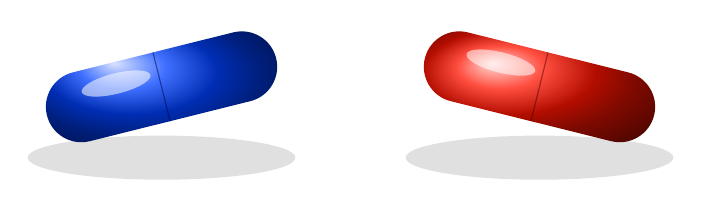
\begin{tikzpicture}[thick]

  % ---- soft shadows on the ground ----
  \fill[black!12] (1.6,-0.55) ellipse (1.7 and 0.28);
  \fill[black!12] (6.4,-0.55) ellipse (1.7 and 0.28);

  % ---- blue pill, tilted left ----
  \begin{scope}[shift={(1.6,0.35)}, rotate=14]
    \shade[ball color=blue!75!cyan]
      (-1.05,-0.45) -- (1.05,-0.45) arc (-90:90:0.45)
      -- (-1.05,0.45) arc (90:270:0.45) -- cycle;
    % seam between the two capsule halves
    \draw[blue!30!black, thin, opacity=0.5] (0,-0.45) -- (0,0.45);
    % specular highlight
    \fill[white, opacity=0.55] (-0.55,0.18) ellipse (0.45 and 0.13);
  \end{scope}

  % ---- red pill, tilted right ----
  \begin{scope}[shift={(6.4,0.35)}, rotate=-14]
    \shade[ball color=red!85!orange]
      (-1.05,-0.45) -- (1.05,-0.45) arc (-90:90:0.45)
      -- (-1.05,0.45) arc (90:270:0.45) -- cycle;
    \draw[red!30!black, thin, opacity=0.5] (0,-0.45) -- (0,0.45);
    \fill[white, opacity=0.55] (-0.55,0.18) ellipse (0.45 and 0.13);
  \end{scope}

\end{tikzpicture}
\end{document}
